\errorcontextlines99999
\documentclass[10pt,journal,compsoc]{IEEEtran}
\usepackage[compress]{cite}
\def\citemid{,~}%
\def\citepunct{],~[}% similar to ieee but i do not want breaks
\usepackage[pdftex]{graphicx}
\usepackage{amsmath}
\interdisplaylinepenalty=2500
\usepackage{algorithmicx}
\usepackage{array}
\usepackage[caption=false,font=footnotesize,labelfont=sf,textfont=sf]{subfig}
\usepackage{fixltx2e}
\usepackage{stfloats}
\usepackage{booktabs}
\usepackage{siunitx}
\usepackage[table]{xcolor}
\fnbelowfloat
% \usepackage{dblfloatfix}
%\ifCLASSOPTIONcaptionsoff
%  \usepackage[nomarkers]{endfloat}
% \let\MYoriglatexcaption\caption
% \renewcommand{\caption}[2][\relax]{\MYoriglatexcaption[#2]{#2}}
%\fi
% For subfig.sty:
% \let\MYorigsubfloat\subfloat
% \renewcommand{\subfloat}[2][\relax]{\MYorigsubfloat[]{#2}}
\usepackage{url}
\usepackage[hidelinks]{hyperref}
\usepackage{csquotes}
\usepackage[capitalise]{cleveref}
\crefname{subsection}{Subsection}{Subsections}

\usepackage{siunitx}
\usepackage{amssymb}
\usepackage{listings}

\usepackage[inline]{enumitem}
\newlist{inlist}{enumerate*}{1}
\setlist[inlist]{itemjoin={{, }},itemjoin*={{,~and\space}},label=\;\textsl{\roman*\/)},mode=boxed}
\newlist{orlist}{enumerate*}{1}
\setlist[orlist]{itemjoin={{, }},itemjoin*={{,~or\space}},label=\;\textsl{\alph*\/)},mode=boxed}

\def\T#1{\textsl{Type\nobreakdash-#1}}

\hyphenation{}

\def\todo#1{\textcolor{brown!80!yellow!70!black!90!red}{[\textsc{todo}: \textsf{#1}]}}
\def\note#1{\textcolor{green!80!yellow!70!black!90!red}{[\textsc{note}: #1]}}
\usepackage[style=mmddyyyy,yearmonthsep={/},dayyearsep={/},monthdaysep={/}]{datetime2}
\newcommand*\urldate[2]{\url{#1}\;\textsuperscript{\color{gray}\DTMdate{#2}}}
\newcommand*\footurl[3][]{\footnote{#1\urldate{#2}{#3}}}

\usepackage{tikz}
\usetikzlibrary{decorations.pathreplacing,arrows.meta}

\begin{document}
\title{Code Clone Detection in the Context of Semantically Equivalent Code}

% https://peerj.com/articles/cs-49/
% https://www.arxiv-vanity.com/papers/2002.08653/

\author{Florian~Sihler% ,~\IEEEmembership{Member,~IEEE,}
\IEEEcompsocitemizethanks{\IEEEcompsocthanksitem F.~Sihler is a student at Ulm University.\protect\\
E-mail: \href{mailto:florian.sihler@uni-ulm.de}{florian.sihler@uni-ulm.de}}%
%\thanks{Manuscript received ?? ??, ????; revised ?? ??, ????.
}
\def\markcell{\cellcolor{gray!20!white}}

\makeatletter
\markboth{Journal of \enquote{Aktuelle Themen der Softwaretechnik aus Forschung und Praxis}, February~2021}% ~Vol.~?? before date
{Sihler: \@title}

\IEEEtitleabstractindextext{%
\begin{abstract}
Code clones amount to a significant fraction of today's software system, resulting in a lot of research regarding the identification of duplicated code pieces and yielding a large amount of \textsl{semi-automatic code clone detection tools} (CCDT).
However, only some of those tools claim the capability to identify semantically equivalent code clones that differ in syntax. Furthermore, many CCDTs are unmaintained and undocumented research projects, resulting in challenges when reproducing previous comparative benchmarking results. Moreover, most previous comparisons restrict themselves to one benchmark using \textsl{BigCloneBench}.

This paper aims to do four things by \begin{inlist}
  \item presenting a set of Docker images for a selected set of CCDTs, which eases the reproduction of previous results
  \item benchmarking the selected CCDTs using accepted answers to the Google Code Jam (assuming they are semantically equivalent)
  \item comparing the results with another benchmark of the code of first-semester computer science students
  \item revealing differences in code clones produced by experienced and beginner programmers
\end{inlist}. Besides the students' code used, we make everything available online.
We reveal various problems in reproducing existing code cloning benchmarks and find significant differences in the number of clones detected by different CCDTs.
\end{abstract}

\begin{IEEEkeywords}
Code Clone Detection, Code Clones, Docker, Automation, Benchmark, Google Code Jam
\end{IEEEkeywords}}

\maketitle

\IEEEdisplaynontitleabstractindextext

\IEEEpeerreviewmaketitle

\IEEEraisesectionheading{\section{Introduction}\label{sec:introduction}}


\IEEEPARstart{C}{ode clones} or code duplicates are widespread in software systems amounting to a fraction from~\qtyrange{7}{23}\percent~\cite{roy2009comparison,schulze2010code} or even up to \qty{30}\percent~\cite{wagner2013software,wagner2016functionally,kim2005empirical} of the complete codebase.
Therefore, there exists a lot of research on detecting code clones and mitigating their harmful effects on software maintenance~\cite{juergens2009code}. This research produced a wide
variety of (semi\nobreakdash-)automated tools and techniques thoroughly compared and evaluated by other studies~\cite{roy2009comparison,ain2019systematic}.
However, they \begin{inlist}
  \item differ in their exact definition of what a code clone is
  \item are rather old or restrict themselves to older code
  \item restrict the types of code clones detected to those syntactically equivalent
  \item only use \textsl{BigCloneBench}~\cite{svajlenko2021bigclonebench} as a basis for comparison
\end{inlist}.
Furthermore, many code clone tools are research projects and neither portable nor actively maintained, leading to hardly reproducible results and many links to sites and files that are no longer available combined with no or faulty tutorials.

% \todo{url dates}
Therefore, besides a clear definition of what we consider to be a code clone, this paper aims to achieve four things: \begin{enumerate}
  \item A Docker image\footurl{https://www.docker.com/}{2022-02-13} for each code clone detection tool, locked to the version that we used and automatically running all required manual steps for comparison. They are available at: \urldate{https://github.com/Code-Clone-Detection-Images}{2022-02-13}.
  \item A benchmark of those detection tools focusing on semantic code clones (as defined in \cref{code-clone-types} below) using accepted answers to the \textit{Google Code Jam}~(GCJ).\footurl{https://codingcompetitions.withgoogle.com/codejam/}{2022-02-13} % \todo{Kategorienvergleich mit \cite{gorg2017deriving}}
  \item A comparative benchmark using code of first-semester computer science students to,\ldots
  \item reveal differences and similarities between code written by experienced and by beginner programmers.
\end{enumerate}
% \todo{Problem mit Definition, manche sind klar, manche Schwammig, viele alt. Nutzen \emph{BigCloneBench} die meisten gehen nur bis zu typ-3, last: Overview}
% Forschungsfragen
% \subsection{Overview}
This paper focuses on comparing code clone detection tools confronted with
semantically equivalent code while answering the research questions in \cref{subsec:research-question}.
In addition, \cref{sec:Background} equips the reader with knowledge regarding types of different code clones and standard techniques used by detection tools.
In \cref{sec:Method} we outline our benchmarking procedure, followed by \cref{sec:prep} and \cref{sec:exp} describing the required preparation steps and the
implementation of the experiment whose results are depicted in \cref{sec:results} and discussed in \cref{sec:discussion}.
\cref{sec:related-work} integrates our research into the broader context of code clone detection, associating it with the related work in the field.
Finally, \cref{sec:conclusion} concludes the paper and informs about possible future work.



\section{Background}\label{sec:Background}
For this paper, we use the terminology established by Chanchal Roy~\textsl{et~al.}~\cite{roy2009comparison}.
That is, we define a \textit{code fragment}~(CF) as any continuous sequence of code lines---denoted by the starting and ending line numbers---inside a file.
A \textsl{CF\textsubscript1} is considered to be a \textit{code clone} of another \textsl{CF\textsubscript2} if it is equal in respect to a similarity function \(f\) defined by the clone type below in \cref{code-clone-types}: \(f(\text{\textsl{CF\textsubscript1}}) = f(\text{\textsl{CF\textsubscript2}})\). Multiple code fragments which are code clones of each other (\enquote{clone pairs}) are considered as a \textit{clone group}.

\subsection{Types of Code Clones}\label{code-clone-types}
\textsl{CFs} can be similar in their syntax or their semantics.
We differentiate between four common types of code clones, numbered from \T1 to~\T4 (cf.~\cite{roy2009comparison,10.1145/3381307.3381310}, and Listing~\ref{clone-types-examples}):
\begin{enumerate}
  \item differ only in whitespace, layout, and comments.
  \item differ additionally in identifiers, literals, and types.
  \item differ additionally in some statements.
  \item differ in syntax but perform same computation.
\end{enumerate}
While the first three types are clearly defined in most works and sometimes even subdivided into weak, moderate, and strong candidates~\cite{svajlenko2014towards}, the fourth one is defined loosely in terms of which computations are similar enough to be regarded as a code clone. Furthermore, code clone detection tools that focus on \T4 clones vary in the differences they acknowledge between \T3 and \T4. %---some even use an analog scale defining a smooth transition between those types.

\begin{lstlisting}[float,caption={Example of the four different clone types \protect\T{1\,--\,4} in Java (based on {\cite[Listing 1]{saini2018oreo}} and {\cite[List 3]{wu2020scdetector}}).\bigskip},abovecaptionskip=0pt,language=Java,basicstyle=\ttfamily,numbers=left,frame=single,keywordstyle={[2]{\itshape}},morekeywords={[2]{String}},numberstyle=\sffamily\scriptsize,label=clone-types-examples]
String join(String[] elements) {
  String result = "[";
  int i = 0;
  while(i < elements.length) {
      if(i > 0) result += ", ";
      result += elements[i++];
  }
  return result + "]";
}
String joinType1( String[] elements ) {
  String result = "["; // Comment!
  int i         = 0;
  while ( i < elements.length) {
      if (i > 0) result += ", ";
      result += elements[ i++ ];
  }
  return result + "]";
}
String joinType2(String[] es) {
  String r = "[";
  int count = 0;
  while(count < es.length) {
      if(count > 0) r += ", ";
      r += es[count++];
  }
  return r + "]";
}
String joinType3(String[] es) {
  String r = "";
  for(int c = 0; c < es.length; c++) {
      if(c > 0) r += ", ";
      r += es[c];
  }
  return "[" + r + "]";
}
String joinType4(String[] es) {
  return "[" + helper(es, 0);
}
String helper(String[] es, int i) {
  if(i >= es.length) return "]";
  else if (i > 0)
    return ", " + es[i] + helper(es, i+1);
  else return es[i] + helper(es, i+1);
}
\end{lstlisting}

Additionally to those type-based separations, some researchers classify clones according to their location (i.e., their physical expanse), their attractiveness for refactorings (cf.~\cite{gautam2016various}) and the variations between them (cf.~\cite{gorg2017deriving}).
However, we decided against including those metrics as we focus on detecting \T4 clones and not, for example, on the identification of CFs applicable for refactoring.

% \todo{Different definitions}

% \todo{Young thesis for semantic: \cite{al2021towards}}

\subsection{Code Clone Detection}
\begin{figure}
\resizebox\linewidth!{\sffamily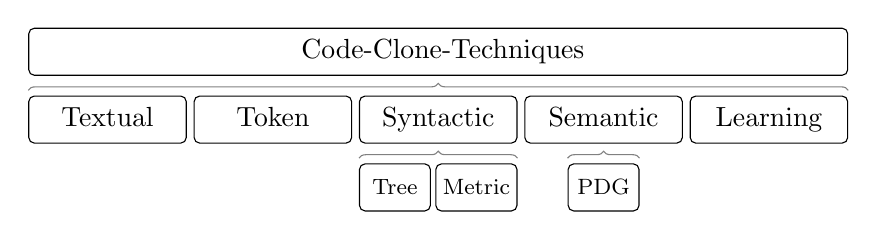
\begin{tikzpicture}[every node/.style={rectangle,draw,rounded corners=2pt,minimum width=2cm,execute at begin node=\strut,inner sep=2.5pt},x=1.05cm]
  \node (0) at (0,0) {Textual};
  \node (1) at (2,0) {Token};
  \node (2) at (4,0) {Syntactic};
  \node (3) at (6,0) {Semantic};
  \node (4) at (8,0) {Learning};

  \node[above=2.5mm,minimum width=10cm*1.05-.5mm*2] (r) at (2.north) {~~Code-Clone-Techniques~~};

  \node[below right,yshift=-2.5mm,minimum width=2cm/2-.1cm] (2a) at(2.south west) {\footnotesize Tree};
  \node[below left,yshift=-2.5mm,minimum width=2cm/2-.1cm] (2b) at(2.south east)  {\footnotesize Metric};

  \node[below,yshift=-2.5mm,minimum width=2cm/2-.1cm] (3a) at(3.south) {\footnotesize PDG};

  \draw[decoration=brace,decorate,gray] ([yshift=.66mm]0.north west) -- ([yshift=.66mm]4.north east);
  \draw[decoration=brace,decorate,gray] ([yshift=.66mm]2a.north west) -- ([yshift=.66mm]2b.north east);
  \draw[decoration=brace,decorate,gray] ([yshift=.66mm]3a.north west) -- ([yshift=.66mm]3a.north east);
\end{tikzpicture}}%
\caption{Code-Clone Technique Classification (cf.~\cite[Figure 1]{10.1145/3381307.3381310}).}
\label{fig:cats}
\end{figure}
The authors Walker, Cerny and Song identify five different techniques used by code clone detection software~\cite{10.1145/3381307.3381310} and specify subcategories as shown in \cref{fig:cats}.
We summarize them briefly below and classify the clone detection tools we consider accordingly in
\cref{lbl:cons-tools}.
\def\expl#1{\item\textit{#1}:}%
\begin{itemize}
  \expl{Textual} approaches are language independent by comparing two CFs using string or lexeme comparison.
  \expl{Token-Based} or lexical approaches convert the source code into a token stream and compare the token sequences.
  \expl{Syntactic} approaches build \textsl{abstract syntax trees}~(AST) from the source code and compare the subtrees directly, or they construct vectors classifying CFs using various metrics and then search for resembling vectors.
  \expl{Semantic} approaches group all attempts on specifically finding \T4 clones. Walker~\textsl{et~al.}~\cite{10.1145/3381307.3381310} identify the use of \textsl{program dependency graphs} (PDGs) to be the most common technique.
  \expl{Learning} approaches use machine learning or similar techniques to detect duplicate CFs. % We do not consider them in this paper.
\end{itemize}
Besides using techniques of these five categories, most code clone detection tools follow the same three step process to identify code clones~\cite{10.1145/3381307.3381310,ain2019systematic}.
First, in the preprocessing stage, they remove irrelevant elements in the source and divide it into units for the comparison (cf.~\cite{kamiya2002ccfinder,rattan2013software}).
Second, in the transformation stage, the remaining source code is transformed into an \textsl{intermediate representation}~(IR) like an AST or the \textit{C Intermediate Language} (CIL\footurl{https://github.com/cil-project}{2022-02-15}).
Regarding the IR used, especially low-level IRs have been shown to be a beneficial format for code clone detection by Caldeira~\textsl{et~al.}~\cite{caldeira2020improving}.
Additionally, the transformation stage is used for the population of arbitrary assisting data structures like PDGs.
Third, in the match detection stage, all transformed CFs are compared to produce a list of clone pairs or clone groups~\cite{roy2009comparison}.

% \cite{10.1145/3381307.3381310} figure 1
% \todo{preprocessing (\cite{kamiya2002ccfinder,rattan2013software}), code representation, and code similarity representation} WOHER KOMMT DAS? teils \cite{roy2009comparison}
% \cite{ain2019systematic}

% \todo{; text based, token based, ast based---auch nachher nochmal anfügen; string-, token-, tree-, semantics-based TODO: intermediate??}

% Klassifikation weiter in am Anfang: \cite{walker2020open}

% not found: \todo{properties auch in Various Code Clone Detection Techniques and Tools: A Comprehensive Survey}

\section{Method}\label{sec:Method}
There already exists a large number of benchmarks regarding code clone detection tools using BigCloneEval~\cite{svajlenko2014towards} which itself is built around BigCloneBench~\cite{svajlenko2021bigclonebench} which in turn relies on the \textsl{IJaDataSet~2.0}~\cite{ijadataset}.
However, the creators of this BigCloneBench separated the collected open-source Java projects based on their syntactical differences and judged their functional similarities by three judges.
While this allows a higher level of confidence in the identified clones and provides an extensive database of larger projects, there are disadvantages:
The identification process is error-prone, expensive, and relatively inflexible---the creation of \textsl{BigCloneBench} required 216 hours of manual validation only for the classification of clones in one language.
Therefore, we have decided to use another dataset for the benchmark, which is more flexible regarding the languages used and the amount of preparation work required.

% \todo{Vorteile: menschlich geprüft und größeres Projekt, nNchteile: genannt}

\subsection{Sources}\label{sec:sources}
Similar to Stefan Wagner~\textsl{et~al.}~\cite{wagner2014detection,wagner2016functionally} we use the accepted answers to the \textit{Google Code Jam}~(GCJ) to provide our experiment with a large set of programs written to solve the same problem---therefore, we regard them as semantically equivalent (cf.~\cite[p.~10]{ComparingProgrammingLanguages2017}).
Like Wagner~\textsl{et~al.}, we restrict the supported languages to \textsl{C} and \textsl{Java} due to the wide variety of code clone detection tools available for those languages. Albeit them being not the most used languages in the GCJ---which are C++ and Python~\cite[Table~5.1]{ComparingProgrammingLanguages2017}---they provide us with thousands of solutions for a lot of problems and therefore with enough data to work with.
We describe the challenges in retrieving those solutions in \cref{accepted-answers-gcj}.


Furthermore, we differentiate our approach from Wagner~\textsl{et~al.} as they only use three CCDTs:
\begin{itemize}
  \item CCCD which we use as well, as described in \cref{lbl:cons-tools} below.
  \item ConQAT\footurl{http://www.conqat.org}{2022-02-15}, an open-source dashboard toolkit which reached its end of live in 2018.
  \item Deckard\footurl{https://github.com/skyhover/Deckard}{2022-02-15} which was only capable of Java code up to version 4 during Wagners' study. In 2018 it got an update to support Java versions 6 and 7.
\end{itemize}
Additionally, we use the exercise code of first-semester computer science students at \textit{Ulm University}\footnote{Please be aware that we are not able to share the used source code files of these first-semester students.} to compare the characteristics of their code with the accepted solutions of the Google Code Jam.
Because those exercises are in Java, we restrict the comparison to this language.
% \todo{Leider können/dürfen wir die Quellen nicht veröffentlichen, deswegen auch nicht reproduzierbar.}
% \todo{Ulm University Kram nicht reprooduzierbar---hinschreiben}

% TODO: Since it is hard to fake correct output with-
% out writing a correct program, we consider all solutions in the repository fulfill the
% requirements to be used as data in this study.
% similar to "Comparing Programming Languages in Google Code Jam"

\subsection{Considered Tools}
\label{lbl:cons-tools}
Each code in either Java or C is analyzed by a set of (semi-)automatic clone detection tools.
This set consists of tools specifically created to detect \T4 clones: \begin{inlist}
  \item \textsl{CCCD}, short for Concolic Code Clone Detection~\cite{6671332}, which is only capable of handling Code written in C
  % \todo{\cite{wagner2016functionally} [use their categories?]}% https://web.archive.org/web/20150921003732/http://www.se.rit.edu/~dkrutz/CCCD/index.html?page=install
  \item \textsl{Oreo}~\cite{saini2018oreo} which is only capable of Java%https://github.com/Mondego/oreo
  \item \textsl{Agec}~\cite{6613854} which is only capable of Java% https://github.com/tos-kamiya/agec2 and https://github.com/tos-kamiya/agec
\end{inlist}.

Furthermore, we employ other tools that specialize on clone types aside from \T4: \begin{inlist}
  \item \textsl{SourcererCC}~\cite{SourcererCC} which we use for Java files
  % \item \textsl{Deckard}~\cite{Deckard} capable of Java and C
  \item \textsl{NICAD}~\cite{cordy2011nicad} which is capable of Java and C% high ranking with oreo
\end{inlist}.
% https://github.com/Mondego/SourcererCC
% tutorial falsch datenbank ist oopslaDB

\begin{table*}
\centering\def\y{\(\checkmark\)}\begin{tabular}{llccccll}
    \toprule
         &        &     &  \multicolumn{2}{c}{Language}    &  & \multicolumn{2}{c}{Technique}\\
    \cmidrule{4-5}\cmidrule{7-8}
    Tool & Author & Year & Java & C & Clone-Type & Category & Strategy \\
    \midrule
    CCCD & Krutz~\textsl{et~al.}~\cite{6671332}               & 2013 &      & \y & \T1\,--\,\T4 & Semantic & Levenshtein Distances of Concolic Information. \\
    Oreo & Saini~\textsl{et~al.}~\cite{saini2018oreo}         & 2018 & \y   &    & \T1\,--\,\T4 & Semantic\footnotemark & Compares metrics of \textsl{CFs}. \\
    Agec & Kamiya~\cite{6613854}                               & 2013 & \y   &    & Mostly \T4 & Semantic & Matches execution paths in Java bytecode. \\
    \midrule
    SourcererCC & Sajnani~\textsl{et~al.}~\cite{SourcererCC}  & 2015 & \y   &   & \T1\,--\,\T3  & Token-Based & Compares the similarity of Tokens \\
    NICAD       & Cordy~\textsl{et~al.}~\cite{cordy2011nicad} & 2009 & \y   & \y & \T1\,--\,\T3 & Syntactic & Uses Flexible Pretty-Printing to compare \textsl{CFs}. \\
    \bottomrule
  \end{tabular}\medskip
  \caption{Short overview of the used code clone detection tools and their important characteristics.}
  \label{tbl:tools}
\end{table*}
\footnotetext{To be precise, Oreo uses Deep-Learning as well but only to specifically classify \T3 and \T4 clones.}

All tools are summarized in \cref{tbl:tools} and are described below in greater detail.
% \todo{Tools noch genauer beschreiben und nach \cref{fig:cats} Kategorisieren}
\begin{figure}
\centering{\sffamily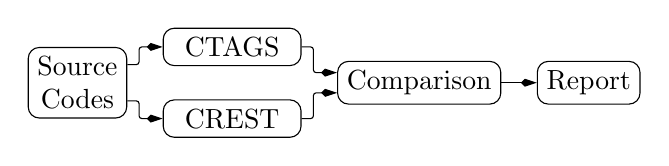
\begin{tikzpicture}[k/.style={rectangle,draw,rounded corners,minimum width=1.25cm,minimum height=4mm,align=center}]
  \node[k] (s) at (0,0) {Source\\Codes};
  \node[k,right=4.5mm,minimum width=1.75cm] (ctags) at (s.north east) {CTAGS};
  \node[k,right=4.5mm,minimum width=1.75cm] (crest) at (s.south east) {CREST};
  \node[k,right=4.5mm] (comp) at (s.east-|crest.east) {Comparison};
  \draw[-Kite,rounded corners=1pt] (s.20) -- ++(1.5mm,0) |- (ctags.west);
  \draw[-Kite,rounded corners=1pt] (s.-20) -- ++(1.5mm,0) |- (crest.west);

  \draw[-Kite,rounded corners=1pt] (ctags.east) -- ++(1.5mm,0) |- (comp.173);
  \draw[-Kite,rounded corners=1pt] (crest.east) -- ++(1.5mm,0) |- (comp.187);

  \node[k,right=4.5mm] (rep) at (comp.east) {Report};
  \draw[-Kite] (comp) -- (rep);
\end{tikzpicture}}
\caption{Major steps of CCCD-CCDT (based on~\cite[Figure 1]{6671332}).}
\label{fig:steps-cccd}
\end{figure}


\subsubsection{CCCD}
\label{expl:cccd}We selected CCCD (short for Concolic Code-Clone Detection) for two reasons. First, because it is a prominent \T4 code clone detection tool, and second, due to its interesting and novel approach of using concolic information~\cite{krutz2013code}.

CCCD uses a twofold analysis of source code by analyzing it using a modified version of \textsl{CREST} (a concolic test generation tool for the C language) and \textsl{CTAGS} (a tool to extract function information from source code).
Because CREST is restricted to the C language and function-level (i.e., it does not generate distinguishable concolic information inside of a function), CCCD itself is only capable of analyzing function clones inside of C programs.

After the preparation, CCCD compares the concolic output of CREST based on the function information provided by CTAGS by calculating the Levenshtein distance~\cite{levenshtein1966binary,al2021towards}. CCCD outputs a report of all function combinations alongside their distance (see \cref{fig:steps-cccd}).

Regarding the classification of clones, Krutz~\textsl{et~al.} state that they identified scores greater than 35 yielding too many false positives. Therefore, we decided on using the same (recommended) threshold for clone detection.

\subsubsection{Oreo}\label{sec:oreoX}
We selected Oreo by Saini~\textsl{et~al.}~\cite{saini2018oreo} as it is a relatively recent addition to the pool of available code-clone detection tools.

Because comparing all clone pairs is a very expensive task, Oreo employs two preselection phases to eliminate unlikely clone pairs. The first preprocessing phase \enquote{Size Similarity Sharding} eliminates all clones differing greatly in size. Further, it produces shards that partition the input based on the method size.
The second preprocessing phase \enquote{Semantic Similarity} compares so-called action tokens (e.g., all methods called, field accesses,~\ldots) to reduce the set of potential clone pairs additionally.

After those two phases, Oreo makes use of feature vectors generated from a large set of metrics (e.g., counting the number of Numerical literals) to differentiate \T{1\,\&\,2} clones from the \enquote{Twilight Zone} (\T{3\,\&\,4} clones).

In order to identify \T{3\,\&\,4} clones, Oreo uses a pretrained neural network (based on a Siamese architecture~\cite{baldi1993neural}).

\begin{figure}
\centering{\sffamily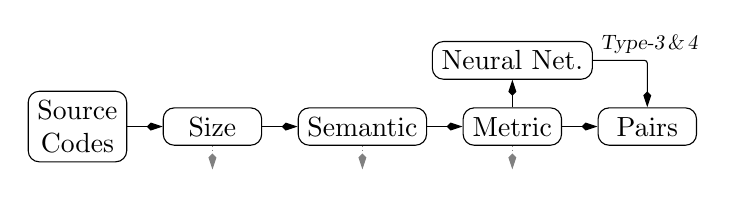
\begin{tikzpicture}[k/.style={rectangle,draw,rounded corners,minimum width=1.25cm,minimum height=4mm,align=center}]
  \node[k] (s) at (0,0) {Source\\Codes};
  \node[k,right=4.5mm] (si) at (s.east) {Size};
  \node[k,right=4.5mm] (se) at (si.east) {Semantic};
  \node[k,right=4.5mm] (me) at (se.east) {Metric};
  \node[k,right=4.5mm] (cl) at (me.east) {Pairs};
  \node[k,above=3.5mm] (nn) at (me.north) {Neural Net.};
  \node[above right,scale=.75] at(nn.east) {\T{3\,\&\,4}};

  \draw[-Kite] (s) -- (si);
  \draw[-Kite] (si) -- (se);
  \draw[-Kite] (se) -- (me);
  \draw[-Kite] (me) -- (cl);
  \draw[-Kite,densely dotted,gray] (si.south) -- ++(0,-3mm);
  \draw[-Kite,densely dotted,gray] (se.south) -- ++(0,-3mm);
  \draw[-Kite,densely dotted,gray] (me.south) -- ++(0,-3mm);
  \draw[-Kite] (me) -- (nn);
  \draw[-Kite,rounded corners=1pt] (nn) -| (cl);
\end{tikzpicture}}
\caption{Major steps of the Oreo-CCDT (based on~\cite[Figures 1 \& 2]{saini2018oreo}). Arrows pointing down represent possible rejection phases.}
\label{fig:steps-oreo}
\end{figure}

\subsubsection{Agec}\label{sec:agec}
The approach of Agec differs, as it compiles source files to Java bytecode in order to perform static analysis by extracting and matching n-grams (in this case, sub-strings of a given length of execution sequences, cf.~\cite{kondrak2005n}). The primary goal of the prototype implementation is the identification of potential refactoring locations by detecting semantic clone pairs~\cite{6613854}. Hence, it does not differentiate between clone types and only reports if something is a potential code clone (of any type) by the process illustrated in \cref{fig:steps-agec}.

\begin{figure}
\centering{\sffamily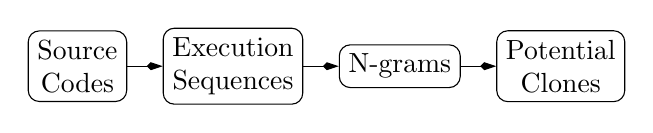
\begin{tikzpicture}[k/.style={rectangle,draw,rounded corners,minimum width=1.25cm,minimum height=4mm,align=center}]
  \node[k] (s) at (0,0) {Source\\Codes};
  \node[k,right=4.5mm] (si) at (s.east) {Execution\\Sequences};
  \node[k,right=4.5mm] (se) at (si.east) {N-grams};
  \node[k,right=4.5mm] (pc) at (se.east) {Potential\\Clones};

  \draw[-Kite] (s) -- (si);
  \draw[-Kite] (si) -- (se);
  \draw[-Kite] (se) -- (pc);
\end{tikzpicture}}
\caption{Major steps of the Agec-CCDT (based on~\cite[Figure 2]{6613854}).}
\label{fig:steps-agec}
\end{figure}

\subsubsection{SourcererCC}\label{SourcererCC}
We chose SourcererCC as it is a state-of-the-art token-based CCDT that \begin{inlist}
  \item is build for scalability
  \item was already used in various code clone benchmarks and studies (cf.~\cite{10.1145/3133908,ain2019systematic,su2016code})
\end{inlist}.

\begin{figure}
\centering{\sffamily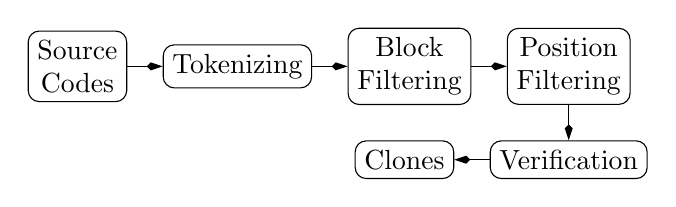
\begin{tikzpicture}[k/.style={rectangle,draw,rounded corners,minimum width=1.25cm,minimum height=4mm,align=center}]
  \node[k] (s) at (0,0) {Source\\Codes};
  \node[k,right=4.5mm] (si) at (s.east) {Tokenizing};
  \node[k,right=4.5mm] (se) at (si.east) {Block\\Filtering};
  \node[k,right=4.5mm] (pc) at (se.east) {Position\\Filtering};
  \node[k,below=4.5mm] (cv) at (pc.south) {Verification};
  \node[k,left=4.5mm] (cp) at (cv.west) {Clones};

  \draw[-Kite] (s) -- (si);
  \draw[-Kite] (si) -- (se);
  \draw[-Kite] (se) -- (pc);
  \draw[-Kite] (pc) -- (cv);
  \draw[-Kite] (cv) -- (cp);
\end{tikzpicture}}
\caption{Major steps of the SourcererCC-CCDT (based on~\cite[Figure 2]{SourcererCC}).}
\label{fig:steps-sourcerercc}
\end{figure}

In order to speed up clone detection, SourcererCC first builds a partial index by using a simple Scanner to identify tokens and blocks in the source files and filtering them according to the tokens these blocks may have in common.
By exploiting sorting, token frequency (similar to natural languages), and previous filters, runtime complexity for the candidate verification gets reduced from quadratic to linear time~\cite{SourcererCC}.
Furthermore, by working with bags-of-tokens (arbitrarily ordered multisets of tokens) which abstract away distances between tokens, SourcererCC claims to be better in identifying \T3-clones than other code clone detection tools (as illustrated in \cref{fig:steps-sourcerercc}).


\subsubsection{NICAD}
NICAD, which is a (loose) acronym for Accurate Detection of Near-miss Intentional Clones---being \T3-clones in the terminology used by us---exploits TXL~\cite{cordy2006txl}, an agile parsing language for source code transformation created by the same authors.

\begin{figure}
\centering{\sffamily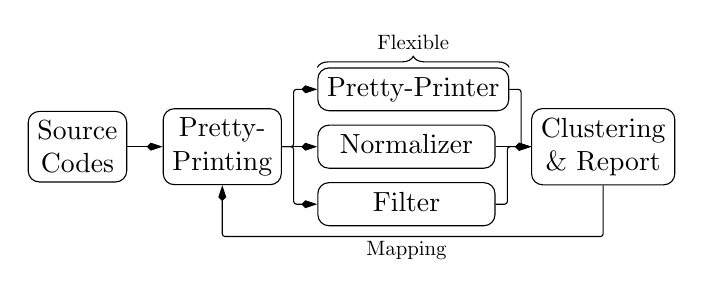
\begin{tikzpicture}[k/.style={rectangle,draw,rounded corners,minimum width=1.25cm,minimum height=4mm,align=center}]
  \node[k] (s) at (0,0) {Source\\Codes};
  \node[k,right=4.5mm] (si) at (s.east) {Pretty-\\Printing};
  \node[k,above right=4.5mm,minimum width=2.25cm] (a) at (si.east) {Pretty-Printer};
  \node[k,right=4.5mm,minimum width=2.25cm] (b) at (si.east) {\vphantom{y}Normalizer};
  \node[k,below right=4.5mm,minimum width=2.25cm] (c) at (si.east) {\vphantom{y}Filter};

  \draw[decoration={brace,amplitude=4pt},decorate] (a.north west) to[edge node={node[above=4pt,scale=.75] {Flexible}}] (a.north east);

  \node[k,right=4.5mm] (d) at (b.east) {Clustering\\\& Report};

  \draw[-Kite] (s) -- (si);
  \draw[-Kite,rounded corners=1pt] (si.east) -- ++(1.5mm,0) |- (a.west);
  \draw[-Kite] (si.east) -- (b);
  \draw[-Kite,rounded corners=1pt] (si.east) -- ++(1.5mm,0) |- (c.west);

  \draw[-Kite,rounded corners=1pt] (a.east) -- ++(1.5mm,0) |- (d.west);
  \draw[-Kite] (b.east) -- (d);
  \draw[-Kite,rounded corners=1pt] (c.east) -- ++(1.5mm,0) |- (d.west);

  \draw[-Kite,rounded corners=1pt] (d.south) -- ++(0,-6.5mm) -| (si.south);
  \node[below=1mm,scale=.75] at(c.south) {Mapping};
\end{tikzpicture}}
\caption{Major steps of the NICAD-CCDT (based on~\cite[Figure 1]{cordy2011nicad}).}
\label{fig:steps-nicad}
\end{figure}

Based on research regarding code clones in HTML~\cite{cordy2004practical}, the first step removes unimportant syntactical elements (like comments) using static pretty-printing rules. Additionally, it enforces a minimum of ten lines for something to be considered a code clone.
Using the pretty printed code, NICAD makes use of three techniques: \begin{inlist}
  \item flexible pretty-printing allowing for splitting statements of different granularities
  \item flexible normalization by (partially) removing identifier names, conditions, and more
  \item flexible code filtering removing configurable statements and parameters
\end{inlist}.
Afterwards, all information is combined and analyzed (searching for longest common subsequences) to form clusters of code clones (as shown in \cref{fig:steps-nicad}).

\subsection{Comparison}
For each problem in the Google Code Jam and each computer science introductory course exercise, we group all accepted solutions by the used language.
Regarding the \textsl{GCJ} we use 100\footnote{We have chosen 100 submissions because some higher rounds of the GCJ only have roughly 120 submissions in the C language. However, our setup and preparation allow for numbers far greater than that.} accepted Java and C solutions for each exercise. Regarding the introductory course, we use all supplied solutions. These have been manually verified for correctness by the author.

We run the tools mentioned above for each group applicable to the respective language and measure all detected clones.
Considering that all solutions of each group solve the same exercise, we expect a very high rate of (potential \T4) clones.

% In the discussion in \cref{sec:discussion}, we then compare the detected clone types and argue for the applicability of these (semi-)automatic clone detection tools.
% Additionally, we examine the differences and similarities between the solutions of the \textsl{GCJ} and those of the introductory course.


% CCCD: Concolic code clone detection % \url{https://ieeexplore.ieee.org/abstract/document/6671332?casa_token=d8G6l4B4ezAAAAAA:OSJ-kNHwVTZKhxVBrPTNcJDbiLWwV_QAZh0UeOx4DPqNnkzlfeSOOUsZTh3vza1xcHnXCZdH4ig}
% Krutz is not available: https://nsuworks.nova.edu/gscis_etd/201/
% \cite{wagner2014detection,wagner2016functionally}
% <(=) 35 => code clone

\subsection{Research Questions}
\label{subsec:research-question}As part of the experiment, we formulate the three following research questions:
\begin{enumerate}[label=RQ\arabic*),leftmargin=*]
  \item \label{rq-1}What are the required setup steps to reproduce previous results and studies?
  \item Are there any differences between the CCDTs specifically written for semantic clones?
  \begin{enumerate}[label=RQ1.\alph*),leftmargin=*,widest=R1.ii)]
    \item Regarding the number of clones detected?
    \item Regarding the speed required to detect these clones?
  \end{enumerate}
  \item Are there differences in code clones found in the GCJ and those found in code by first-semester students?
\end{enumerate}
They are addressed and answered accordingly in the following sections.

% \todo{Klarer die Hypothesen aufschlüsseln}
% Regarding the results, we expect the CCDTs specialized on \T4 clones to perform well, as all solutions should be semantically equivalent (i.e., solving the same problem using a syntactically different approach).

%\todo{We expect type 4 clones to perform very well---same task}
% \todo{Replicateability: Links und Versionen}

\section{Preparation}\label{sec:prep}
This section describes the required steps and challenges in retrieving and preparing the answers to the GCJ, the code of the first-semester students, and the CCDTs.

We decided on the necessity of creating Docker images during the preparation phase, as it turned out, that most CCDTs require a very specific set of dependencies to work.

\subsection{Accepted Answers to the Google Code Jam}
\label{accepted-answers-gcj}
With the shut down of the Google Code Archive in 2016,\footurl{https://code.google.com/archive/}{2022-02-15} Google moved its archive of submitted solutions to its official Google Code Jam site,\footurl{https://codingcompetitions.withgoogle.com/codejam}{2022-02-15} where they are presented in an inscrutable manner~\cite{ComparingProgrammingLanguages2017}.
While there exist publicly available datasets that include parts of GCJ solutions (like the DeepSIM\footurl{https://github.com/parasol-aser/deepsim}{2022-03-01} testing dataset,~\cite{wang2020detecting}) we found a mirror archive containing a large CSV file for each Code Jam\footurl{https://github.com/Jur1cek/gcj-dataset}{2022-03-01} and wrote an extraction script to work with the submitted solutions.\footurl[See for the prepare script named \enquote{GCJ-csv-preparation} in~]{https://github.com/Code-Clone-Detection-Images}{2022-03-14}

Additionally, this extraction script runs in a Docker container and uniformly selects a configurable amount of solutions that have been: \begin{inlist}
  \item validated (so they fit the desired contests)
  \item in case of java-submissions compiled and anonymized\footnote{Each Java class is assigned a new random name consisting of one random uppercase ASCII and 24 random ASCII letters and digits. The number can be increased easily in the source file.} so that they work with Agec, which must be able to compile all sources into a single Java archive
\end{inlist}.

After running the script, we have a folder structure that contains the desired amount of randomly selected and validated solutions for each problem.
Because all other tools are set up so that they require a folder to work with, we can easily use the folder structure as a basis for the experiment without any additional modification (although we ordered the results in the context of this work).

% \todo{Verweis auf google, was die Lösungen nicht mehr frei und einfach zur Verfügung stellt (das Archive bietet ohne klar erkennbares Muster noch die Lösung an, wir verwenden ein Archive auf Github) und beispielsweise CCCD oder Oreo wo die tutorials falsch sind}


\subsection{Preparing the Tools}
Most code clone detection tools are either research projects or commercial closed-source products based on former research projects (like ConQAT).
Therefore, most of them are unmaintained and undocumented or---at least to the best of our knowledge---not available online (we contacted several authors but did not receive any answer).
This segment presents a brief overview of the steps and challenges encountered when preparing the selected CCDTs.

\subsubsection{CCCD}
While CCCD is said to be available online, all provided links do no longer work, so we relied on the internet archive,\footurl[The original link is no longer working: ]{https://web.archive.org/web/20200209173743/http://www.se.rit.edu/~dkrutz/CCCD/index.html?page=install}{2022-02-14} uncovering links to the no longer active Google Code Archive and a no longer working Google Drive link resulting in us having to reconstruct most modifications by hand.
Based on the installation instructions (which did not work), we created---step by step---a Docker image running Fedora 34 with OCaml\footurl{https://ocaml.org/}{2022-02-14} 3.09.0 due to the unavailability of older stable configurations, although the newest version of CCCD was reported to be working on Fedora 14 (released in November 2010).

During the build of the Docker image, we migrate dozens of old OCaml instructions using \texttt{sed} commands, match the required compilers manually, and build old versions of CREST\footurl{https://github.com/jburnim/crest}{2022-02-14} and CTAGS\footurl{http://ctags.sourceforge.net/}{2022-02-14} (which CCCD uses in a modified version, as described in \cref{expl:cccd}) from scratch.

We validate the build process by re-running the test file provided by CCCD and comparing the results automatically.
The produced image can be started by supplying it with a folder containing the source files for the analysis. All other steps are performed automatically by a custom run-script, including the classification of clones which is based on the calculated Levenshtein distances.

% \todo{Darauf eingehen, dass nirgendwo die Bewertungsgrenzen für die \T1 bis \T4 Klone vermerkt sind.}

\subsubsection{Oreo}

Given that Oreo is a recent research project with an evaluated and validated artifact,\footurl{https://github.com/Mondego/oreo/releases}{2022-03-01} constructing a Docker image is a reasonably simple task. We automate all manual steps (like the creation of a virtual environment) and reduce all configuration options to environment variables wherever necessary.

However, although there is an artifact, reproducing the results of Oreo proved to be difficult~\cite{wang2020detecting} with a \enquote{bug} of Oreo being that it is unable to detect \textit{any} clones.
For example, the default configuration of Oreo was not able to deal correctly with nested folders (missing a crucial \texttt{null}-check), which in term meant that all nested folders failed silently.\footnote{Oreo reports an error if and only if all folders are nested as it is unable to process any file in this case.}
Furthermore, most steps are run asynchronous and do not notice if they are finished. Leading to many waits in the run script to ensure that one step is completed before the next one starts.
All required modifications can be found in the GitHub-Repository: \urldate{https://github.com/Code-Clone-Detection-Images}{2022-02-13}.

\subsubsection{Agec}
While Agec appears to be discontinued (the successor Agec2\footurl{https://github.com/tos-kamiya/agec2}{2022-03-01} is marked as such), building a Docker image turned out to be uncomplicated.
We automated all required steps and manually searched through the source code in order to identify essential but undocumented flags (like the diagnostic flag, which prints out metrics regarding the detected n-grams).

Because Agec needs to compile all Java sources to Java bytecode, we extended our extraction script of \cref{accepted-answers-gcj} to only select files that can be compiled inside of the Agec Docker image. In order to prevent problems with duplicated classes or references to different classes with the same name, it further scrambles all class identifiers (consistently over multiple files of the same submission).
Please note that we do not guarantee that the output is collision-free. However, with randomly chosen 25-character long class names, we expect them to be different---ensuring collision-free names is outside of the scope of this paper.

In order to validate the Docker image, we re-run Agec on the example code presented with the original paper~\cite{6613854} and validate each step with the expected output automatically.

\subsubsection{SourcererCC}
In the context of the DéjàVu project~\cite{10.1145/3133908}, the authors of SourcererCC built a virtual machine that contains all necessary scripts and preconfigured databases for SourcererCC to run.
We adapted those configurations and reverse-engineered the required database setup to create a fully automatic script (running docker-compose\footurl{https://docs.docker.com/compose/}{2022-03-01}) which prepares and configures all required files dependent on the input.

Furthermore, we run SourcererCC with all 12 projects of the original paper (during the build process of the container) and automatically validate it with the expected output produced by the virtual machine.

\subsubsection{NICAD}
NICAD is the only tool we consider that is capable of analyzing both considered languages.
For the Docker image, we first build TXL and install NICAD afterwards.\footurl{https://www.txl.ca/}{2022-03-01}
However, since the original version of NICAD is no longer available, we use the most up-to-date version, which is \mbox{\textit{NiCad~6.2}}. After reading the tutorial on the website, everything worked without any problem.
% \todo{refine this and the other texts}

\subsection{Configurations}\label{configuration}
We used the standard or recommended configuration for each CCDT but built the Docker images with customizability in mind. For the experiment, we used the following settings.

For \textsl{CCCD} there is not a lot to configure. We chose the same Levenshtein distance threshold (35) as recommended by the authors~\cite{6671332}. Because the filtering mechanisms of \textsl{Oreo} are flexible, there as well is not much to configure that affects the clones found---we kept the 15 token minimum for shards.
We configured \textsl{Agec}s n-grams to the default size of six and limited the search to one branch.
Regarding \textsl{SourcererCC} we reconstructed the configuration from the artifact, allowing for all C language file extensions.
\textsl{NICAD} (NiCad~6.2) got configured to detect clone types \T{2\&3} with a \enquote{Difference Threshold} of \qty{30}\percent\ for clusters. Furthermore, it limits clones to sizes between 10 and 2500 lines (which is the recommended range).


\subsection{Conclusion}
This section as a whole answered \ref{rq-1} by presenting all of the major steps required to get the selected CCDTs running. The individual repositories at \urldate{https://github.com/Code-Clone-Detection-Images}{2022-02-13} contain all the required steps to build, test, and run each image.

\section{Experiment}\label{sec:exp}
In this section, we describe the steps of the experiment alongside all of the problems encountered and how we have dealt with them. We use all tools as prepared in the previous preparation phase described in \cref{sec:prep}.

\subsection{Selected Tasks}
\label{subsec:selected-task}This subsection briefly describes, justifies and explains how many samples we took from which problem set.

\subsubsection{Google Code Jam}
For the GCJ solutions, we have selected 100 random submissions for each language from each of the following five problems. We selected these problems due to the high number of participants and either because they have been used in other benchmarks with GCJ submissions or because they are fairly recent:
\begin{itemize}
  % \itemsep\smallskipamount
  \item \textsl{2016 Qualification Round:\quad Counting Sheep}\\*
  The introductory qualification challenge of the GCJ 2016, \enquote{Counting Sheep} was attempted by 26\,612 participants, \qty{95}\percent\ of which solved both available datasets (for seven and eight points each).
  \textit{For both C and Java, we use the small problem set (chosen at random).}
  \item \textsl{2016 Round 1A:\quad The Last Word}\\*
  \enquote{The Last Word} is the challenge of one of the three variants of the first round after the Qualifications. \enquote{The Last Word} was solved by over 10\,000 participants, \qty{94}\percent\ of whom were able to solve both---the small dataset for nine and the large dataset for eleven points.
  \textit{For both C and Java, we use the large problem set (chosen at random).}
  \item \textsl{2016 Round 1C:\quad Senate Evacuation}\\*
  Similar to \enquote{The Last Word}, \enquote{Senate Evacuation} is part of a variant of the first round after the Qualifications. It got solved by roughly 6\,000 participants, \qty{90}\percent\ of whom were able to solve both datasets: the small one for eight and the large one for ten points.
  \textit{For both C and Java, we use the small problem set (chosen at random).}
  \item \textsl{2017 Round 1B:\quad Steed 2: Cruise Control}\\*
  \enquote{Steed 2: Cruise Control} was the introductory challenge of the first round after the Qualifications in the GCJ 2017. It offered two datasets for eleven and fourteen points. From more than 8\,000 participants, \qty{92}\percent\ solved both datasets.
  \textit{For both C and Java, we use the large problem set (chosen at random).}
  \item \textsl{2020 Qualification Round:\quad Vestigium}\\*
  As the introductory challenge of the GCJ in the year 2020, \enquote{Vestigium} was attempted by 43\,280 participants and got solved by \qty{90}\percent.
  \textsl{We chose the only dataset available (which was worth seven points) for both languages}.
\end{itemize}
We refrained from using challenges in the higher rounds due to the low number of remaining participants. For example, a lot of round three challenges have only just about 100--200 participants summed over all languages---a large portion of which failed the datasets.
Nevertheless, we consider the first rounds to be a sufficient basis for the tests.
% \todo{darüber schreiben warum keine hohen und ds wir mit den niedrigen challenges zufrieden sind. selbst für die qualification, auch als kleinen vergleich untereinander}

% \todo{make them available as part of the github group}

\subsubsection{University Students}
Due to the fact that we can not openly share the solutions of the first-semester computer science students, we keep the explanation of the selected tasks briefly.
We chose the following exercises:
\begin{itemize}
  \item Taxi-Class: The students had to implement a Taxi class with precisely defined methods to drive and refill the Taxi and a method to pay the driver.
  \item Combinations: the students were tasked with printing all fixed-length combinations of a given array.
  \item Binary Tree: Given an exact definition of a format to print a binary tree, the students were tasked with reproducing this format for balanced binary trees, given as an array.
\end{itemize}
For each task, we used the solutions of all students that passed a manual verification by the authors.

\begin{table}
  \centering\resizebox\linewidth!{\begin{tabular}{l rr rrr}
    \toprule
    & \multicolumn{2}{c}{CCCD} & \multicolumn{3}{c}{NICAD} \\
    \cmidrule(r){2-3} \cmidrule{4-6}
    Round & Total & Clones & Total & Classes & Clones \\
    \midrule
    Counting Sheep & 118 & 70 & 160 & 0 & 0 \\ % TODO: short solution
    The Last Word & 34 & 15 & 148 & 0 & 0 \\
    Senate Evacuation & 51 & 27 & 214 & 2 & 2 \\
    Steed 2: Cruise Control & 126 & 82 &  150 & 1 & 1 \\
    Vestigium & 271 & 170 & 169 & 12 & 12 \\
    \bottomrule
  \end{tabular}}\medskip
  \caption{Clones detected in C language submissions to the GCJ. \textit{Total} refers to the total number of possible \enquote{comparison units} detected (i.e. possible clone candidates). For NICAD, \textit{Classes} represents identified clone groups, which do not differ for this table (i.e., every clone group holds one clone pair)}
  \label{tbl:clones-c}
\end{table}

\begin{table*}
   \def\k#1{}%
    \centering\resizebox\textwidth!{\begin{tabular}{lc rrr rrr cc c rrr}
      \toprule
                &          & \multicolumn{3}{c}{Oreo} & \multicolumn{3}{c}{Agec} & & \multicolumn{3}{c}{NICAD} \\
      \cmidrule(r){3-5} \cmidrule{6-8} \cmidrule{10-12}
       Exercise & Samples & Blocks & \T{1\&2} & \T{3\&4} & n-grams & distinct & clones  & SourcererCC & Total & Classes & Clones \\
    \midrule
    Counting Sheep & small & 224 & 6\k3 & 104\k{46} & 1812 & 1149 & 39 & 0 & 224 & 2 & 2 \\
    The Last Word & large & 212 & 6\k3 & 141\k{67} & 1985 & 1573 & 69 & 0 & 212 & 7 & 9 \\
    Senate Evacuation & small & 392 & 21\k1 & 244\k{62} & 7092 & 3432 & 139 & 0 & 392 & 12 & 35 \\
    Steed 2: Cruise Control & large & 230 & 1\k0 & 77\k{33} & 7316 & 3231 & 115 & 0 & 230 & 2 & 6 \\
    Vestigium & all & 181 & 8\k3 & 282\k0 & 2915 & 1595 & 173 & 0 & 181 & 8 & 20 \\
    \bottomrule
  \end{tabular}}\medskip
  \caption{Clones detected in Java language submissions to the GCJ. For Oreo it is possible to get more clones than there are block, because blocks may share different subsets with other blocks. Agec differentiates between \enquote{distinct} n-grams as only those are considered for code clones.}
  \label{tbl:clones-java}
\end{table*}

\subsection{Used Setup}
We performed all experiments and built all images on a Manjaro Linux 64 bit distribution\footurl{https://manjaro.org/}{2022-02-15} using Docker version 20.10.12 build \texttt{\href{https://github.com/docker/cli/tree/e91ed5707e038b02af3b5120fa0835c5bedfd42e}{e91ed5707e}} and at least 16 gigabytes of free RAM available at all times. We run only one CCDT at a time.
The required time was measured using the POSIX command-line tool \texttt{time}.\footurl{https://linux.die.net/man/2/time}{2022-03-04}

\section{Results}\label{sec:results}
In this section, we present the results from the experiment, executed as described in the previous section.
We describe the results obtained by the GCJ and first-semester student submissions and address the fact that SourcererCC could not identify any clone in the test set.

% todo: compare with file size
\begin{table*}
  \def\k#1{}% TODO: vasted percenages
  \centering\resizebox\textwidth!{\begin{tabular}{lc rrr rrr cc c rrr}
    \toprule
              &          & \multicolumn{3}{c}{Oreo} & \multicolumn{3}{c}{Agec} & & \multicolumn{3}{c}{NICAD} \\
    \cmidrule(r){3-5} \cmidrule{6-8} \cmidrule{10-12}
     Exercise & Samples & Blocks & \T{1\&2} & \T{3\&4} & n-grams & distinct & clones  & SourcererCC & Total & Classes & Clones \\
    \midrule
    Taxi Class   & 50 & 280 & 8\k3& 212\k{76}& 16118 & 4624 & 132 & 0 & 280 & 14 & 40 \\
    Combinations & 21 & 58  & 6\k{10}& 58\k{100} & 24138 & 1667 & 11 & 0 & 58  & 1  & 1 \\ % uses tree recursion
    Binary Tree  & 17 & 99  & 10\k{10}& 16\k{16} & 1908 & 856 & 105 & 0 & 99 & 5 & 10 \\
    \bottomrule
  \end{tabular}}\medskip
  \caption{Code clones detected in the submissions of the first-semester computer science students.}
  \label{tbl:clones-first-semester}
\end{table*}

\begin{table}
  \centering\begin{tabular}{l cc}
    \toprule
    Problem & CCCD & NICAD\\
    \midrule
    Counting Sheep          & 0:39 & 0:13 \\
    The Last Word           & 0:36 & 0:11 \\
    Senate Evacuation       & 0:48 & 0:06 \\
    Steed 2: Cruise Control & 0:36 & 0:11 \\
    Vestigium               & 0:44 & 0:14 \\
    \bottomrule
  \end{tabular}\medskip
  \caption{The time (in minutes) required by each tool for the given analysis of C sources. This excludes the build time of the docker image, but includes the startup time of the container.}
  \label{tbl:required-time-c}
\end{table}

\begin{table}
  \centering\resizebox\linewidth!{\begin{tabular}{l cccc}
    \toprule
     Exercise/Problem & Oreo &  Agec & SourcererCC & NICAD\\
    \midrule
    Counting Sheep & 3:05 & 0:21 & 0:16 & 0:04\\
    The Last Word & 3:04 & 0:17 & 0:14 & 0:05 \\
    Senate Evacuation & 3:04 & 0:49 & 0:14 & 0:05 \\
    Steed 2: Cruise Control & 3:04 & 0:19 & 0:16 & 0:04\\
    Vestigium & 3:03 & 0:33 & 0:14 & 0:04 \\
    \midrule
    Taxi Class   & 3:10 & 0:31 & 0:33 & 0:03 \\
    Combinations & 3:07 & 0:36 & 0:15 & 0:01 \\
    Binary Tree  & 3:01 & 0:10 & 0:20 & 0:01 \\
    \bottomrule
  \end{tabular}}\medskip
  \caption{The time (in minutes) required by each tool for the given analysis of Java sources. For Oreo the time is heavily influenced by fixed wait times in order to ensure sequential execution of asynchronous operations (amounting to roughly one minute).} %  \todo{note times are already arbirary}
  \label{tbl:required-time-java}
\end{table}


% \todo{compare with \cite{caldeira2020improving}}
For the GCJ solutions, the results are presented in \cref{tbl:clones-c,tbl:clones-java} for the C language and Java language submissions respectively, revealing significant differences in clones detected.

The times required for each analysis are in \cref{tbl:required-time-c,tbl:required-time-java} for C language and Java language submissions. However, they should only give an approximate understanding as all CCDTs did run completely inside a Docker container, leading to potential overhead.

The results for the analysis of the university students are listed in \cref{tbl:clones-first-semester}.
Due to the low sample size, the authors verified each identified potential clone by hand.

\begin{table}
  \centering\begin{tabular}{l lll lll}
    \toprule
                            & \multicolumn{3}{c}{C} & \multicolumn{3}{c}{Java} \\
    \cmidrule(r){2-4}\cmidrule{5-7}
    Exercise/Problem        & min & max & avg & min & max & avg\\
    \midrule
    Counting Sheep          &  8 & 227 & 57 & 28 & 310 & 62\\
    The Last Word           &  14 &440 & 52 &  19 & 824 & 56 \\
    Senate Evacuation       &  22 & 434 & 85 & 39 & 2050 & 123\\
    Steed 2: Cruise Control & 17& 1238 & 57  & 19& 558 & 59\\
    Vestigium               &  10&  1672 & 82&  14& 1707  & 76 \\
    \midrule
    Taxi Class & & & & 56 & 178 & 98 \\
    Combinations & & & & 17 & 71 & 36 \\
    Binary Tree & & & & 34 & 233 & 105 \\
    \bottomrule
  \end{tabular}\medskip
  \caption{Sizes (in lines of code) of the solutions submitted to the GCJ Problems and the university exercises. Only the selected samples are included.}
  \label{tbl:file-sizes}
\end{table}


\subsection{Google Code Cam}
\subsubsection{C Submissions}
Looking at \cref{tbl:clones-c} the difference between clones found by CCCD and NICAD is enormous.
However, when paired with the solutions sizes in \cref{tbl:file-sizes} it becomes apparent that some complete solutions to the GCJ are smaller than the minimum size threshold of NICAD to be detected as a clone (which is ten lines).
Furthermore, most GCJ submissions use a rather generic and short main-method while writing the solution as a standalone function~--- leading to even shorter potentially cloned CFs.
Therefore, NICADs approach of limiting code clones by their (pretty-printed) line size does fail.

CCCD---on the other hand---does not have this limit. Therefore it matches clones regardless of their initial size.
Nevertheless, looking more closely at the raw information (which is part of the aforementioned GitHub organization as well) reveals that the minimum Levenshtein distances are rather high, while the maximum distance is rather low (resulting in a large amount of detected \T4 clones, that NICAD does not claim to detect).
For \enquote{Counting Sheep} the minimum distance is \num{19}, the maximum distance is \num{39} with everything lower or equal to \num{35} being regarded as a clone.
Consequently, modifying the threshold of CCCD and NICAD has drastic effects on the number of code clones discovered.

\subsubsection{Java Submissions}
The results for the Java submissions vary widely as well. While no CCDT labeled all submissions as code clones of each other, Oreo is at the top with most clones discovered (besides \enquote{Steed 2: Cruise Control}).
Just like with the C submissions, NICAD falls short due to its line minimum for potential clones, eliminating a lot of potential candidates.
The code clones discovered by Agec do heavily depend on the configured n-gram size (see \cref{configuration}).
However, we decided that the testing of different configurations is best left for potential future work, as it exceeds the scope of this paper.
The problem with SourcererCC will be discussed separately in \cref{problem:SourcererCC}.

\subsection{University Students}
Regarding the analysis of the submissions of the university students, Oreo proved to be surprisingly accurate, with no false positives (to the author's knowledge).
The low clone count of Oreo regarding the \enquote{Binary Tree} exercise is due to the multitude of completely different strategies in solving this problem.
While some students chose a naive approach of nested for-loops, some implemented balanced binary trees as linked data structures, while others made use of binary-tree-specific characteristics.
All CCDTs failed in assigning these approaches as clones.

Nevertheless---at least for now---it is not to be expected that an arbitrary CCDT can understand the similarity in these completely different approaches.

% \todo{explain nicad low for combinations}
NICAD failed in identifying a lot of clones in the \enquote{Combinations} exercise due to its line limit and because its pretty printing has problems with comparing recursive with non-recursive solutions (as it does not translate one format into the other).

\subsection{SourcererCC}\label{problem:SourcererCC}
When we did encounter that SourcererCC was unable to match any clone, we thought of an error and checked each step. However, in the scope of this paper, we were unable to find any error in the setup.
We had no problem reproducing \textit{exactly} the results of the original paper and got the same results inside of the supplied virtual machine.
Therefore, by sharing the complete configuration, we leave this problem as potential future work.
% and exclude SourcererCC in the following discussion

\section{Discussion}\label{sec:discussion}
In this section, we discuss the results of the experiment presented in \cref{sec:results} in the context of the research questions (\cref{subsec:research-question}), compare both benchmarks, and consider the threats to validity.

\subsection{The Research Questions}

\subsubsection{RQ2) Are there any differences between the CCDTs specifically written for semantic clones?}
We can find a significant difference in the number of code clones detected and a mild difference in the speed of the programs.
Looking at \cref{tbl:clones-c} the amount of clones detected is significant---for all exercises, most clones detected by CCCD are very close to the \num{35}-threshold, meaning that they are very likely to be \T4-clones.
Even more, all semantic code clone tools detect more clones overall, compared to the \T3 CCDTs.

However, interpreting the required time with \cref{tbl:required-time-c,tbl:required-time-java} is more difficult.
While Oreo needs the most time, Agec is sometimes quicker than SourcererCC, albeit specifically designed for sematic clone detection.
This might be either due to the overhead of using a Docker container~\cite{li2017performance} or
simply because of the manual waits required to synchronize otherwise asynchronous tasks.

Nevertheless, in general, semantic clone detection tends to be a lot slower (especially for larger datasets~\cite{SourcererCC}) than \T{1\,--\,3} detection.

\subsubsection{RQ3) Are there differences in code clones found in the GCJ and those found in code by first-semester students?}
In theory, there should be no difference in \T4 clones detected, as both---experts and beginners---have to implement a program with the same functionality. However, interpreting the clones by the CCDTs, there appear to be (relatively) more clones in the solutions by the first-semester university students.
This difference might be explained by \begin{orlist}
  \item the limited knowledge of the beginner programmers limiting their solutions to the concepts presented in the lecture
  \item the solutions to the task being \enquote{more obvious} as in the GCJ
  \item students working together and sharing their ideas
\end{orlist}.
In order to test these hypotheses in future studies, we share anonymized analysis information of the students' submissions.

\subsection{Threats to Validity}
There exists a wide variety of threats to validity. In the following, we explain each of them and describe any counteraction we have taken.
% We separate the validity into four parts, assessing


\subsubsection{Reliability}
Because not all tools did run out of the box, we had to recreate and update a lot of source files by hand. While we have tested each image either automatically or manually,
we can not guarantee that all CCDTs worked as originally intended (e.g., with SourcererCC).
Additionally, we can not rule out possible interactions with newer language features of both Java and C.

Furthermore, most CCDTs allow for a lot of configurations~\cite{wang2013searching}. For example, Agec allows to configure the size of the n-grams, and CCCD can be interpreted widely based on the calculated Levenshtein Distances.

To counteract these problems, we make everything---apart from the used solutions of the first-semester computer science students---available online to replicate every single step of the study.\footurl{https://github.com/Code-Clone-Detection-Images}{2022-02-13}

\subsubsection{Internal Validity}
The internal validity of an experiment describes to what degree of confidence the
causal relationships between the experiments in \cref{sec:exp}, the results in \cref{sec:results}, and the discussion in \cref{sec:discussion} are not influenced by other factors.

In the context of the used solutions, we have one major threat.
We have no group of experts analyzing the GCJ submissions to be real semantic clones~\cite{svajlenko2014towards}, which means that---at least in theory---different submissions doing different things could be accepted by the GCJ as valid solutions for the same problem.

However, similar to Back and Westman, we argue for the following:
\blockquote[cf.~{\cite[p.~10]{ComparingProgrammingLanguages2017}}]{Since it is hard to fake correct output without writing a correct program, we consider all solutions in the [GCJ] repository [to] fulfill the
requirements to be used as data [\ldots]}
% That is, we assume that even if two programs differ in the exact functionality they implement, in order to pass the datasets of the GCJ they must at least have

We exclude the solutions of the first-semester students from this threat, as they have been selected and verified by hand. However, as only one person checked all of them, they are applicable to the potential internal threat of a human error.


\subsubsection{External validity}
The external validity describes the generalizability and transferability
of the presented findings to other source codes and CCDTs.

As every CCDT works differently, we can make no statement on the performance of other detection tools (even those using the same techniques).
Furthermore, all submissions to the GCJ and the computer science course are rather short (cf.~\cref{tbl:file-sizes}), especially when compared with large projects in the industry, and written by only one or two persons---not large teams. Moreover, due to the time constraint, we considered only a low number of submissions as well.
Additionally, the solutions have been written in a short amount of time with no maintainability in mind,\footnote{The first-semester computer science students had a week to work on each exercise collection in a team of two.} possibly encouraging the use of repetitive patterns (e.g., reusing the same mechanism to split and join arrays over and over again) or the \enquote{first solution that comes to mind.}
% \todo{most sind rauskopiert für generische Sachen (getLongArr)}


Therefore, the generalizability of our findings regarding the detected clone rates is limited. Nevertheless, we still assessed the capability of the selected CCDTs regarding the detection of code clones in general. In theory (accounting for the internal validity of the experiment),
all submissions should be at least \T4 clones of each other. However, we have shown that none of the selected CCDTs was capable of coming close to this expectation.

\subsubsection{Construct Validity}
Construct validity is concerned with interpreting what the identified clone types really represent. This is of concern, as especially the definition of \enquote{The Twilight Zone}~\cite{saini2018oreo}---being the \T{3 and 4} clones---varies slightly between researchers.

We mitigated this by choosing a definition in \cref{code-clone-types} which is consistent with all tools considered. Furthermore, all CCDTs encountered used the functionality of the CF as a guideline to differentiate between \enquote{clones} and \enquote{no-clones}.

\section{Related Work}\label{sec:related-work}
This section integrates the contribution of this paper into the larger context of related fields and related research on \mbox{(semi-)}automatic code clone detection.
We have split the related work into two parts: \begin{inlist}
  \item research concerning CCDTs themselves
  \item research concerning the comparison and evaluation of CCDTs
\end{inlist}.

\subsection{Code Clone Detection}
We did---by far---not benchmark each CCDT there is~\cite{ain2019systematic}.
In the following, we present a brief overview of some significant CCDTs and justify for each of them why we did not select them for this work.

\subsubsection{Deckard}
Deckard~\cite{Deckard} is a syntactic CCDT that is built to scale well for larger projects (just like SourcererCC as described in \cref{SourcererCC}) by using characteristic vectors.
Furthermore, it is already used in several code clone benchmarks~\cite{wagner2014detection,10.1145/3381307.3381310} (cf.~\cref{sec:sources}).

However, we have decided against Deckard as it can only understand and work with Java code up to version 7, which we can neither guarantee for the GCJ nor the first-semester students.

\subsubsection{LICCA}
LICCA~\cite{vislavski2018licca} focuses on identifying code clones written in different languages by using the SSQSA platform (short for Set of Software Quality Static Analysers,~\cite{budimac2012ssqsa}) as a basis.
With this premise, LICCA exceeds the scope of this work as we only compared CCDTs detecting clones in the same language.

\subsubsection{D\textsc{y}CLINK}
The authors of \textsl{D\textsc{y}CLINK}~\cite{su2016code} use a different terminology by searching for \enquote{code relatives}---code fragments with similar execution behavior---instead of the four clone types that we have agreed on in is this work.
Additionally, \textsl{D\textsc{y}CLINK} works similar to Agec (see \cref{sec:agec}) but relies on subgraph matching instead of comparing n-grams.
Due to the restricted time frame of this work, we chose against the integration of this CCDT.

\subsubsection{SCDetector}
The SCDetector CCDT~\cite{wu2020scdetector} uses token sequences to identify semantic clones.
While we wanted to include the SCDetector in our study, neither its sources nor any kind of executable format seems to be available online (the GitHub-Repository only contains the results from the paper).
Additionally, none of our emails asking about the SCDetector have been answered by the authors.
Therefore, including SCDetector was not possible.

\subsubsection{CCFinder}
CCFinder (written in the year 2000) is a rather old CCDT~\cite{kamiya2002ccfinder}, created by Kamiya, Kusumoto, and Inoue.
It uses tokens and is capable of understanding six different languages (including C and Java).
However, we were unable to obtain a running instance of CCFinder, which was capable of either a reasonably modern version of Java or C.

\subsubsection{Other Research on CCDTs}
Besides those CCDTs, research exists to use semantic code clones to identify obfuscated code~\cite{SHENEAMER2018405} exemplifying the applicability of dependency graphs.

Wang~\textsl{et~al.}~\cite{wang2020detecting} analyze the usage of neural nets (similar to those used by Oreo as described in \cref{sec:oreoX}) in the context of BigCloneBench and the GCJ, revealing great potential in learning CCDTs.

\subsection{Comparison and Evaluation}

Using NICAD, Roy and Cordy~\cite{roy2008empirical} evaluate further metrics of code clones in several projects.
On a larger scale, Ain~\textsl{et~al.}~\cite{ain2019systematic} conduct a systematic review on the different mechanisms employed by CCDTs, which is only one of several studies and surveys on code clone detection techniques~\cite{gautam2016various,rattan2013software,shobha2021code,lei2022deep,8668015}.

In his dissertation \enquote{Towards Semantic Clone Detection, Benchmarking, and Evaluation}, the author Al-Omari analyzes semantic clones~\cite{al2021towards}, develops new approaches to identify cross-language clones using intermediate languages, and creates a new kind of benchmark by mining Stack Overflow\footurl{https://stackoverflow.com/}{2022-03-02} for \T4 clones.
In another work of his, he further analyzes code cloning in Games, revealing no difference in clone types and frequency within the same gaming engine while identifying close to no code reuse between different engines~\cite{al2016code}.

Besides these studies, Pate~\textsl{et~al.} analyze the evolution of code clones, improving the scientific understanding of their characteristics~\cite{pate2013clone}.

\section{Conclusion}\label{sec:conclusion}
With this paper, we present a set of Docker images that each contain a specific semi-automatic code clone detection tool.
We use those images to run benchmarks on the accepted submissions to the Google Code Jam and code of first-semester computer science students.
Furthermore, we analyze and compare the produced results identifying the advantages of semantic code clone detection tools (especially Oreo).

Nevertheless, it should be noted that while some research suggests strong evidence that code clones are harmful~\cite{juergens2009code},
not all research considers every clone to be bad. For example, Kapser and Godfrey suggest that as many as \qty{71}\percent\ of all clones have a positive impact on the maintainability of a software system~\cite{kapser2008cloning}.
However, settling this debate is outside of the scope of this paper.

\subsection{Future Work}
There is a lot of potential future work.
\textbullet~One could adapt and include all CCDTs described and referenced alongside the related work in \cref{sec:related-work} in order to extend this kind of comparative and reproducible benchmark.
\textbullet~Additionally, it would be interesting to replicate and extend the comparison of code written by \enquote{experienced programmers}, and \enquote{beginners}, potentially revealing interesting patterns in code clones and code reuse.
This replication could include the examination of SourcererCC, which did not work in the context of our code clone detection benchmark.
\textbullet~Regarding the number of possible configurations (\cref{configuration}), it would be interesting to analyze how to tune the CCDTs to work better with a large number of small source codes.
% Ein frohes wuff wuff an die Gemeinde. -- Hunde vor dem Fenster
% Use functional languages

\appendices

% you can choose not to have a title for an appendix
% if you want by leaving the argument blank
% \section{}
% Appendix two text goes here.


\section*{Acknowledgments}
The author would like to thank Michael Stegmaier and Denis Neumüller for their feedback and support during the writing of this thesis. Furthermore, he expresses his gratitude to Prof. Dr. Matthias Tichy for allowing me to write this paper.
% TODO: auch dem Vortrag von Herrn(?) Juergens danken

% Can use something like this to put references on a page
% by themselves when using endfloat and the captionsoff option.
\ifCLASSOPTIONcaptionsoff
  \newpage
\fi

\bibliographystyle{IEEEtran}
\bibliography{references.bib}

% \begin{IEEEbiographynophoto}{Florian Sihler}
% Biography text here.
% \end{IEEEbiographynophoto}

\end{document}


